
\section{Problema A - Estimación mediante polinomios cuadráticos}
Se quiere estimar la edad de una muestra en la que la proporción $N_{14_c}$ es $0.8705$ a partir de los datos en la tabla:


\begin{table}[H]
	\centering
	\begin{tabular}{llll}
		\hline
		i & $N_{14C}$ & Edad & Rango \\ \hline
		0 & 0.78   & 2050 & 10    \\
		1 & 0.80   & 1850 & 10    \\
		2 & 0.82   & 1650 & 10    \\
		3 & 0.84   & 1450 & 10    \\
		4 & 0.86   & 1250 & 10    \\
		5 & 0.88   & 1050 & 10    \\
		6 & 0.90   & 870  & 5     \\
		7 & 0.92   & 690  & 5     \\ \hline
	\end{tabular}
\end{table}


Determine su edad utilizando el mejor polinomio de interpolación de Lagrange de orden 2 posible, dando la expresión explícita del polinomio interpolador. Justifique su respuesta. (En este apartado hay que entender \textit{mejor} en el sentido de que la estimación tendrá un error menor).

\subsection{Análisis}

\subsubsection{Teoría}

\paragraph{Definición}
La idea central de la interpolación de Lagrange es construir un polinomio 

\begin{equation}
	L_n(x) = \sum_{k=0}^{n} l_k(x) y_k(x)
\end{equation}

dado los puntos:

$$P = \{~ (x_k, y_k) \mid y_k = f(x_k)~ \}_{k=0}^{n}$$

Las funciones $l_k(x)$ son a su vez polinomios con la condición:


\begin{equation}
	l_k(x) = 
	\begin{cases}
		1, & x = x_k \\
		0, & x \neq x_k	
	\end{cases}  
\end{equation}

Se puede representar cada $l_k(x)$ mediante el siguiente producto:

\begin{equation}
	l_k(x) = \prod_{\substack{i = 0 \\ i \neq k}}^{n} \frac{ (x - x_i) }{ (x_k - x_i)}
\end{equation}

\newpage

\subsubsection{Algoritmo}

La implementación de la interpolación de Lagrange se ha hecho mediante el siguiente código:

\lstinputlisting[language=Python, firstline=4, lastline=44]{../../code/methods/lagrangian_interpolation.py}

\newpage

\subsection{Resolución}

\subsubsection{Programación}

Para realizar esta tarea primero generamos todos los polinomios de orden 2.

\paragraph{Generación de polinomios}\label{gen_polynomials}

Los polinomios de orden 2 se generan con la función "generar\_polinomios":

\lstinputlisting[language=Python, firstline=47, lastline=64]{../../code/methods/lagrangian_interpolation.py}

Esto nos dará 6 polinomios, pues tenemos 8 puntos.	

\newpage 

\subsubsection{Polinomios generados vs muestras}

Una vez obtenidos los polinomios, un buen primer paso es tener una visualización gráfica. 

\begin{figure}[H]
	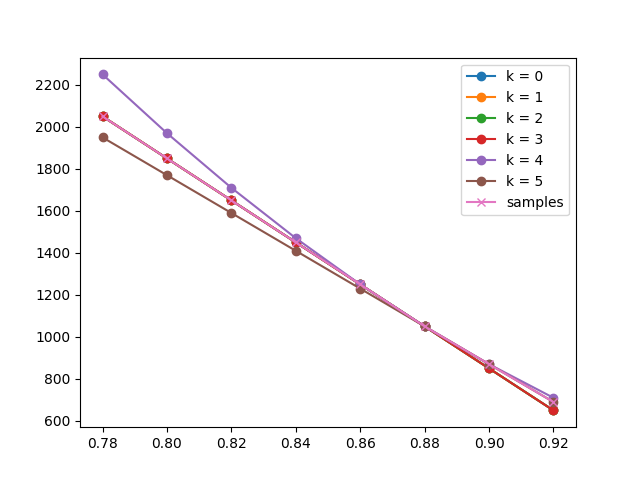
\includegraphics[width=\linewidth]{figures/figure1.png}
	\caption{Gráfica polinomios orden 2 y la muestra}
	\label{fig:interp_cuad}
\end{figure}

Se puede ver claramente que los polinomios tienen menor divergencia con los datos alrededor del punto 0.88.



Lo siguiente es ver cual polinomio ($P(x)$) tiene menor desviación.

Para ello calcularemos el RMSE (root mean square error) y el MAE (mean average error): 

\begin{equation}
	RMSE = \sqrt{ \frac{1}{N} \sum_{k=0} (y_k - p_k)^2 }
\end{equation}

\begin{equation}
	MAE = \frac{1}{N} \sum_{k=0} |{y_k - p_k}|
\end{equation}

donde:
$$ p_k = P(x_k) $$



\begin{table}[htbp]
	\centering
	\csvreader[
	tabular=|c|c|c|,
	table head=\hline \textbf{\#} & \textbf{RMSE} & \textbf{MAE}\\\hline,
	late after last line=\\\hline,
	]{data/errors01.csv}{}{\csvlinetotablerow}
\end{table}


\paragraph{}
Vemos que el polinomio con menor desviación es el polinomio de orden 2 que inicia en k = 1. 


\subsubsection{Resultado}

Generamos la edad estimada por cada polinomio para el valor $0.8705$. 

\begin{table}[htbp]
	\centering
	\csvreader[
	tabular=|c|c|,
	table head=\hline \textbf{\#} & \textbf{Age} \\\hline,
	late after last line=\\\hline,
	]{data/age01.csv}{}{\csvlinetotablerow}
\end{table}

Esto nos da que la edad estimada por el polinomio $P_1$ es:

$$
	P_1(0.8705) = 1144.999999999999 \approx{1145}
$$

